\chapter{Appendiks A}
\label{vco-frekvens}
\section*{VCO frekvens}

Frekvensen på den VCO som anvendes i volumenkontrollen, se afsnit \ref{volumenkontrol-simulering-vco}, er afhængig af flere komponenter. Som tidligere nævnt kan den deles op i to blokke én integrator og én schmidt-trigger. 

\begin{figure}[h]
\centering
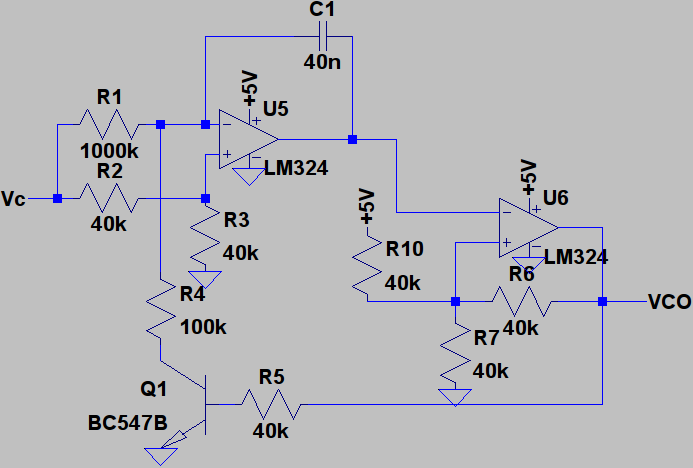
\includegraphics[width=\textwidth]{teknisk/volumenkontrol/vco.png}
\caption{Diagram over VCO'en}
\label{fig:appendiks-vco}
\end{figure}

\subsection*{Schmidt-trigger}

For at opstille et udtryk for frekvensen skal triggerniveauerne for schmidt-triggeren bestemmes, dette gøres vunder den antagelse at et højt udgangs niveau på U6 har samme spænding som forsyningen. Udfra ligning \ref{equ:appendiks-vco1} kan $"$Lower triggerlevel$"$ beregnes.

\begin{equation}
\label{equ:appendiks-vco1}
V_L = \frac{\frac{1}{\frac{1}{R_7} + \frac{1}{R_6}}}{R_{10} + \frac{1}{\frac{1}{R_7} + \frac{1}{R_6}}} \cdot V_{CC} = \frac{R_7 \cdot R_6}{R_{10} \cdot R_6 + R_{10} \cdot R_7 + R_7 \cdot R_6} \cdot V_{CC}
\end{equation}

Hvis de tre modstande $R_6$, $R_7$ og $R_{10}$ gøres ens, kan ligningen yderligere reduceres, se ligning \ref{equ:appendiks-vco2}.

\begin{equation}
\label{equ:appendiks-vco2}
V_L = \frac{R \cdot R}{R \cdot R + R \cdot R + R \cdot R} \cdot V_{CC} = \frac{1}{3} \cdot V_{CC}
\end{equation}

Udfra ligning \ref{equ:appendiks-vco3} kan $"$Upper triggerlevel$"$ beregnes.

\begin{equation}
\label{equ:appendiks-vco3}
V_U = \frac{R_{10}}{\frac{1}{\frac{1}{R_7} + \frac{1}{R_6}} + R_{10}} \cdot V_{CC} = \frac{R_{10} \cdot (R_7 + R_6)}{R_{10} \cdot R_6 + R_{10} \cdot R_7 + R_7 \cdot R_6} \cdot V_{CC}
\end{equation}

Når de tre modstande $R_6$, $R_7$ og $R_{10}$ gøres ens, kan ligningen yderligere reduceres, se ligning \ref{equ:appendiks-vco4}.

\begin{equation}
\label{equ:appendiks-vco4}
V_U = \frac{R \cdot (R + R)}{R \cdot R + R \cdot R + R \cdot R} \cdot V_{CC} = \frac{2}{3} \cdot V_{CC}
\end{equation}

\subsection*{Integrator}
Integratoren op- og aflader kondensatoren $C_1$, dette bliver gjort gennem de to modstande $R_1$ og $R_4$. Med udgangspunkt i den ideelle operationsforstærker, er det klar at spændingen på de to indgange er ens og at operationsforstærkeren vil sikre dette. Det betyder at spændingen på de to indgange kan beregnes med udgangspunkt i $V_{\mathrm{minus}}$

 Når udgangen på $U_6$ er lav vil transistoren $Q_1$ ikke være ledende og der vil ikke løbe strøm gennem $R_4$. Dette vil betyde at al den strøm der løber gennem $R_1$ vil lade $C_1$ op. Når udgangen på $U_6$ er høj vil transistoren $Q_1$ være ledende og der vil løbe en strøm gennem $R_4$. Dette vil betyde at al den strøm der løber gennem $R_1$ vil løbe til stel gennem $R_4$. Strømmen gennem $R_4$ større end strømmen gennem $R_1$, dette skyldes at der også løber strøm fra kondensatoren til stel, det er denne strøm der aflader kondensatoren.